%-----------------
% Header
%-----------------
\documentclass[
a4paper,                % Papierformat A4
12pt,										% Schriftgr��e 12pt
oneside, 								% Zweiseitiges Layout [oneside]
titlepage,              % Titleseite verwenden
headsepline,            % Trennlinie zum Seitenkopf Bereich headings
bibliography=totoc,     % Das Literaturverzeichnis in den TOC
listof=totoc, 					% alle Listen in das Inhaltsverzeichnis
cleardoublepage=plain
]{scrbook}

\bibliographystyle{alphadin}

%-----------------
% Packages
%-----------------
\usepackage[ngerman]{babel}
\usepackage{textcomp}
\usepackage[T1]{fontenc}
\usepackage[latin1]{inputenc}
\usepackage{lmodern}
\usepackage{lscape}
\usepackage{rotating}
\usepackage{tocbasic}
\usepackage{color}
%\usepackage{palatino}
%\usepackage{mathpazo}
%\usepackage{courier}
% left = innen, right = au�en
\usepackage[a4paper, left=4cm, right=3cm, top=4cm, bottom=4cm]{geometry} 

\usepackage{graphicx, amsmath, longtable, booktabs, color, listings, makeidx, pdfpages, subfigure, amsfonts}
\usepackage{float}
\usepackage[pdftex,
	hyperindex=true,
	plainpages=false,
	hypertexnames=true,
	bookmarks=true,
	bookmarksnumbered=true,
	pdfhighlight=/O,
	linkcolor=black,
	citecolor=black,
	filecolor=black,
	menucolor=black,
	urlcolor=black,
	colorlinks=true,
	pdftitle={Projekt 1: STL},
	pdfauthor={Alexander Miller},
	pdfsubject={Dokumentation: Parametric Programming Teil 1},
	pdfstartpage=1]{hyperref}
	
\hyphenation
{
	soft-ware-m�-�i-gen
	kryp-to-gra-phi-schen
	kryp-to-gra-phi-scher
	Ein-weg
	Hash-funk-ti-o-nen
	Pro-to-kol-le
}
	
% Formatierung f�r Code-Listings setzen:
\lstset{basicstyle=\scriptsize\ttfamily,
		keywordstyle=\bfseries\color[rgb]{0.07, 0.21, 0.45},
		keywordstyle=[2]\color[rgb]{0.3, 0.4, 0.5},
		commentstyle={\color[gray]{0.5}\textit},
		stringstyle={\textit},
		xleftmargin=0.5cm, xrightmargin=0cm, framerule=1pt,
		showstringspaces=false, breaklines=true, breakatwhitespace=true,
		numbers=left, numberstyle=\tiny, stepnumber=1, numbersep=0.2cm,
		frame=lines,
		aboveskip=\bigskipamount, belowskip=\bigskipamount,
		framexleftmargin=0.5cm,
		tabsize=4,
		escapeinside={<ref>}{</ref>}}
%--------------------------------------
%   Metainformation
%--------------------------------------
\newcommand{\art}{Angewandte Informatik}
\newcommand{\titel}{Konzeption und Entwicklung einer CD-Tauschb�rse mit \\Ruby on Rails}
\newcommand{\untertitel}{\empty}
\newcommand{\autor}{Christian Bunk \\ Alexander Miller \\ Christian Sandvo� \\ Antonia Ziegler}
\newcommand{\hochschule}{Hochschule f�r Technik und Wirtschaft Berlin}
\newcommand{\fachgebiet}{Angewandte Informatik}
\newcommand{\erstgutachter}{Prof. Dr. Albrecht Fortenbacher}
\newcommand{\datum}{Abgabedatum: 08.01.2012} % durch Abgabedatum zu ersetzen
\newcommand{\ort}{Berlin}


	
%--------------------------------------
%   Dokumentenbeginn
%--------------------------------------
\begin{document}

%--------------------------------------
%   Titelseite
%--------------------------------------
\begin{titlepage}
	\pdfbookmark[-1]{\titel}{Marke}
	% Titelblattkopf
	\titlehead{
		\begin{flushright}
			
\includegraphics[width=0.45\textwidth]{images/HTW_Logo_rgb.jpg}
		\end{flushright}
	}
	\subject{\art \\ Systementwicklung und Frameworks\\ } % Art der Arbeit
	\title{\titel}% Titel der Arbeit
	\subtitle{\untertitel}% ggf. Untertitel
	\author{\autor}% Verfasser
	\date{\datum}% Datum
	\publishers{\erstgutachter}% Betreuer
	\maketitle %erzeugt die Titelseite
\end{titlepage}

%--------------------------------------
%   Seitennummerierung
%--------------------------------------
\pagenumbering{Roman}

%--------------------------------------
%   Abstract und Kurzfassung
%--------------------------------------
%Inhaltsverzeichnis:
\tableofcontents
%\addcontentsline{toc}{chapter}{Inhaltsverzeichnis}
%Abbildungsverzeichnis:
%\listoffigures
%\addcontentsline{toc}{chapter}{Abbildungsverzeichnis}
%Tabellenverzeichnis:
%\listoftables
%\addcontentsline{toc}{chapter}{Tabellenverzeichnis}
%Listingverzeichnis:
%\lstlistoflistings
%\addcontentsline{toc}{chapter}{Listingsverzeichnis}




\pagenumbering{arabic}

\chapter{Einleitung}
\label{sec:Einleitung}

In der Softwaretechnik wird unter dem Begriff Framework ein Ordnungsrahmen verstanden, innerhalb dessen die Entwickler eine Anwendung erstellen. Das Ziel ist die Definition einer einheitlichen Struktur mittels komponentenbasierten Entwicklungsans�tzen sowie die Vereinfachung der Entwicklung durch die Verwendung von zur Verf�gung stehenden Frameworks-Bestandteilen. Im Laufe der Lehrveranstaltung ''Systementwicklung und Frameworks'' wurden die Prinzipien der unterschiedlichen Frameworks wie zum Beispiel EJB und .NET vorgestellt und diskutiert. Als Pr�fungsleistung muss ein Projekt erfolgreich realisiert werden, wobei jede Gruppe von vier bis f�nf Personen die Anwendung mit einem ausgew�hlten Framework entwickeln m�ssen. 

In der vorliegenden Ausarbeitung handelt es sich um eine Dokumentation zum Projekt, wobei eine CD-Tauschb�rse konzipiert und implementiert wurde. Wie in der Aufgabenstellung bzw. im Pflichtenheft definiert (Anhang A.1) wurde eine Rich-Applikation (RIA) modelliert und entwickelt, wobei die meisten Funktionalit�ten nicht von Hand, sondern durch die Verwendung von Framework-Komponenten realisiert wurden. Die Gruppe besteht aus vier Personen (Christian Bunk, Alexander Miller, Christian Sandvo�, Antonia Ziegler) und entwickelt das Projekt mit dem Framework ''Ruby on Rails''. 

Ruby on Rails ist ein Framework f�r Webapplikationen, welches in der Programmiersprache Ruby entwickelt wurde. Model-View-Controller (MVC) Architektur erm�glicht eine Isolation der Businesslogik von der graphischen Benutzeroberfl�che und gew�hrleistet das ''don't repeat yourself'' (DRY) Prinzip. 

Der SourceCode wird mit Git (https://github.com/christianb/SE-FW) verwalten. Hierzu wird die online Plattform GitHub als zentrales Repository verwendet, die sowohl die aktuellen Aufgaben (Issues) als auch die Meilensteine verwaltet. Um eine Arbeitsgrundlage zu erschaffen, haben alle Gruppenmitglieder sich das grundlegende Wissen �ber das ausgew�hlte Framework angeeignet. Wie die geforderten Funktionalit�ten im Einzelnen implementiert sind, kann den folgenden Kapiteln entnommen werden. An dieser Stelle muss noch erg�nzt werden, dass alle gestellten Anforderungen erf�llt wurden.

\chapter{Ruby-on-Rails Framework}
\label{sec:Ruby on Rails Framework}

Ruby On Rails (Rails) ist ein Web-Framework welches auf der Programmiersprache Ruby basiert. Ruby ist eine Objektorientierte Programmiersprache. Anweisungen werden nicht durch ein Semikolon abgeschlossen sondern durch einen Zeilenumbruch. Jede Rails Anwendung hat eine feste Ordnerstruktur und verfolgt das Prinzip ''Convention Over Configuration''. Was bedeutet das der Konfigurationsaufwand durch einhalten von Konventionen so gering wie m�glich gehalten werden soll. Zus�tzlich zu allen erstellten Controllern wird auch ein so genannter Application-Controller erstellt. Alle weiteren Controller sind Unterklassen von diesem und erben daher auch alle Methoden die darin deklariert wurden. Im n�chsten Abschnitt sind die wichtigsten Konventionen n�her erl�utert.
\section{Rails-Konventionen}
\label{KOnventionen}
Wie oben erw�hnt verfolgt Rails das Konzept ''Convention Over Configuration''. Darunter fallen z.B. die Namenskonventionen welche besagen, dass die Namen der Controller m�glichst im Plural benannt werden und Models im Singular. Des Weiteren wird die Schreibweise von Variablen- und Klassennamen geregelt. Durch diese Konventionen weiss Rails welcher Controller zu welchen Modell geh�rt, sowie welche Views zu einem Controller. Dadurch entf�llt die explizite Zuweisung zwischen den einzelnen Komponenten. Die Methoden im Controller werden Actions genannt. Zu jeder Action gibt es meist eine View welches �quivalent zur Bezeichnung der Action benannt ist. Sobald einen View und eine Action den gleichen Namen haben, wird beim Aufruf dieser automatisch die entsprechende View geladen.
\section{Model-View-Controller (MVC)}
\label{MVC}
Das Rails-Framework ist nach dem Model-View-Controller Konzept aufgebaut. Dabei dient das Model zur Kommunikation mit der Datenbank. Au�erdem sorgt es durch Validierung daf�r, dass Daten im korrekten Format in die Datenbank geschrieben werden. Die Views sind die HTML-Seiten, welche dem Nutzer angezeigt werden. Sie dienen zur Anzeige der Daten aus der Datenbank oder dem Erfassen von Nutzereingaben mit Hilfe von Formularen bzw. Eingabefeldern. Der Controller ist der Vermittler zwischen der View und dem Model. Er empf�ngt Daten von der View und sendet sie an das Model weiter. Umgekehrt werden Daten vom Model �ber den Controller der View zur Verf�gung gestellt.
\section{Don't Repeat Yourself (DRY)}
\label{DRY}
DRY beschreibt das ''Don't Repeat Yourself'' Konzept. Dies bedeutet das so wenig wie m�glich Code dupliziert wird. Zur Einhaltung dessen gibt es in Rails einigen Vorkehrungen. Als erstes w�ren da die Helper-Methoden zu nennen. Dies sind Methoden welche oft dazu genutzt werden, h�ufig genutzten Code durch Schl�sselw�rter zu ersetzen. Die Helper-Methoden werden meist in den Views verwendet um dort HTML-Code zu generieren. Ein oft verwendeter Helper ist beispielsweise ''link-to'', welcher den aus HTML bekannten Link-Tag generiert.

Ein weiterer Punkt ist die Definition des Seitenlayouts. Das Layout legt die Darstellung bzw. das Aussehen der HTML-Seiten fest. Dabei kann ein globales, f�r alle Seiten g�ltiges Layout definiert werden oder auch Layout-Vorlagen f�r spezielle Seiten definiert werden. Das Layout welches mit ''application.html.erb'' benannt wird, ist f�r alle Seiten g�ltig. Falls ein anderes Layout verwendet werden soll, muss diese explizit eingebunden werden. Ansonsten wird immer das in der Datei ''application.html.erb'' definierte genutzt. Das gleiche gilt auch f�r den Application-Controller. Hier definierte Methoden sind in allen anderen Controllern verf�gbar und m�ssen dadurch nicht in jedem Controller separat implementiert werden.

Seit der Version 3.1 von Rails, wird standardm��ig jQuery als Javascript Framework verwendet. Auch hier gibt es eine globale Datei (application.js) auf die aus allen Views zugegriffen werden kann. Javascript Code wird in der Regel nicht in den Views eingef�gt, sondern es wird auf die zu ver�ndernden HTML Elemente durch dessen IDs oder Klassen zugegriffen. Dies dient den Prinzip des Unobtrusive (unaufdringlich) Javascript und erh�ht die Lesbarkeit des Codes der Views. Eine weitere Neuerung der Version 3.1, ist die Asset-Pipeline. Darin werden die CSS und JavaScript Dateien gespeichert. Diese werden dann, vor Auslieferung an den Browser komprimiert, um die zu �bertragene Datenmenge zu verringern und dadurch die Zugriffszeit zu erh�hen.

\section{Object-Relation-Mapper (ORM)}
\label{ORM}
Um bei Rails Objekte in einer Datenbank zu speichern, kommt der Object-Relation-Mapper ActiveRecord zum Einsatz. Dabei werden die Tabellen als Klasse gesehen, die Zeilen als Objekt und die Spalten sind die Objekt-Attribute. Durch den ORM m�ssen keine SQL-Statements mehr geschrieben werden, sondern f�r den Zugriff auf die Datenbank werden Methoden genutzt. Beim erstellen einer Tabelle werden von Rails automatisch Methoden generiert. Eine Klasse hat unter andren die Methoden ''new'' und ''find''. Diese dienen zum erstellen oder finden eines Objekts. Das Objekt besitzt die Methoden ''save'', ''update'' und ''delete''. Diese werden zum Speichern, Aktualisieren und L�schen genutzt.

\chapter{Anwendung}
\label{sec:Anwendung}

\section{Projektmanagement}
\label{sec:Projektmanagement}

Eine der wichtigsten Aufgaben bei der Realisierung eines informationstechnischen Projektes ist das Projektmanagement. Es ist �u�erst wichtig eine genaue Planung sowie die Konzeption durchzuf�hren, damit alle Anforderungen, Termine und der Kostenrahmen eingehalten werden. In den n�chsten Kapiteln wird es beschrieben wie das Projektmanagement erfolgte, wobei intensiv auf die Meilensteinplanung sowie die Versionsverwaltung und Deployment eingegangen wird.

\subsection{Meilensteinplanung}
\label{Meilensteinplanung}

Um das Zeitmanagement zu organisieren, wurde die Meilensteinplanung durchgef�hrt. Es wurde vereinbart, dass bei der Entwicklung der meisten Funktionalit�ten immer zwei Gruppenmitglieder beteiligt sein m�ssen, um bei krankheitsbedingten Ausf�llen eines Gruppenmitglieds die Entwicklung fortsetzen zu k�nnen. 

\begin{figure}[ht]
\centering
		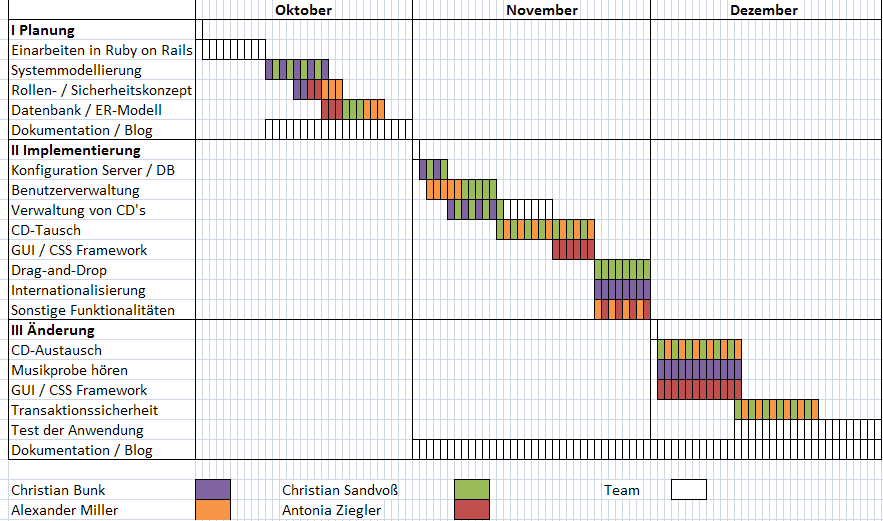
\includegraphics[height=7.2cm]{images/pm.png}
	\caption[Meilensteinplanung]{Meilensteinplanung}
	\label{fig:Meilensteinplanung}
\end{figure}

Dar�ber hinaus wurde es bestrebt, die Konzeption sowie die Systemmodellierung als Gruppenarbeit durchzuf�hren. F�r diese Zwecke wurden w�chentliche Termine (dienstags 12:00-14:00 und donnerstags 11:15 - 12:30) vereinbart. An diesen Terminen wurden in Rahmen einer Gruppenarbeit sowohl die aufgetretenen Schwierigkeiten gel�st, die w�chentliche Pr�sentation vorbereitet als auch der weitere Projektverlauf diskutiert.

\subsection{Versionsverwaltung von Quellcode}
\label{Versionsverwaltung von Quellcode}

F�r die Quellcode-Verwaltung wurde eine GitHub-Repository verwendet. Dabei wurde an das Branching-Modell orientiert, die in ( http://nvie.com/posts/a-successful-git-branching-model/) vorgestellt wird. 

\begin{figure}[ht]
\centering
		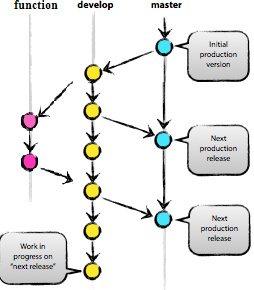
\includegraphics[height=7cm]{images/verlauf.png}
	\caption[Git - Function, Develop und Master Branches]{Git - Function, Develop und Master Branches}
	\label{fig:git1}
\end{figure}

Dabei wird folgende Strategie verfolgt: Als erstes werden zwei Branches angelegt \textit{develop} und \textit{master}. Die eigentliche Entwicklung geschieht auf dem \textit{develop} Branch und lediglich die Zwischenversionen, die eine neue und vor allem fehlerfreie Implementierung einer zus�tzlichen Funktionalit�t beinhalten, werden auf den \textit{master} Branch gelegt. Durch das Erstellen von weiteren Branches f�r die jeweilige Funktionalit�t kann weiterer Komfort bei der Entwicklung erreicht werden. Jede zus�tzliche Funktionalit�t wird dabei separat Entwickelt, so dass eine Aufteilung der Aufgaben sowie die anschlie�ende Zusammenf�hrung der Quelltexte ohne Einschr�nkungen und Probleme erfolgen k�nnen. Wenn eine Funktion fertig gestellt worden ist, wird diese ins \textit{develop} Branch kopiert. Falls mehrere Funktionalit�ten im \textit{develop} Branch getestet und die identifizierten Fehler behoben wurden, wird die Anwendung ins \textit{master} Branch gemergt. Bei der Einhaltung des vorgestellten Modells sieht die Quellcode-Verwaltung wie folgt aus:

\begin{figure}[ht]
\centering
		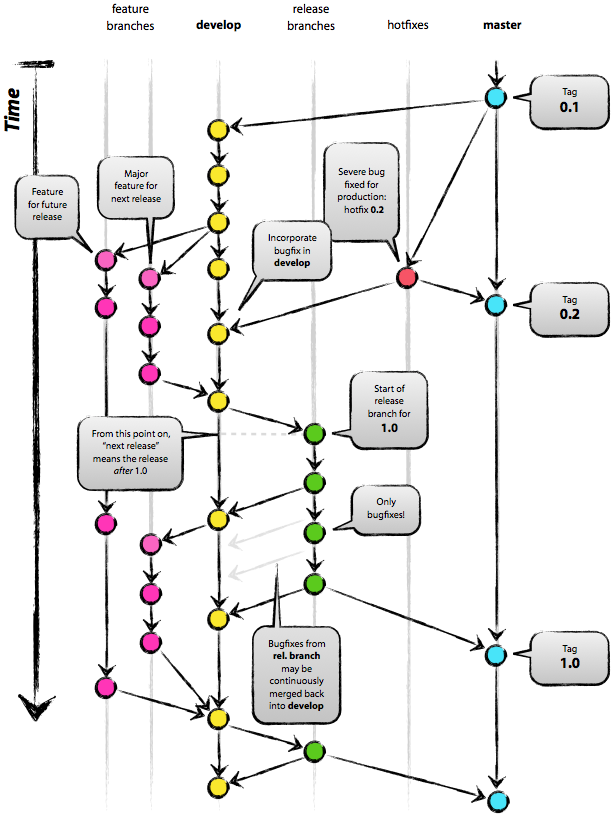
\includegraphics[height=12cm]{images/gitfull.png}
	\caption[Quellcodeverwaltung mit Git]{Git - Feature und Develop Branches}
	\label{fig:git3}
\end{figure}

\subsection{Deployment}
\label{Deployment}

\textbf{Christian Bunk}
%Da die Anwendung auf einem Webserver zur Verf�gung gestellt werden soll, wurde dieser eingerichtet. Daf�r wurde auf den uns zur Verf�gung stehenden Server, als erstes die ben�tigte Software installiert. Um �berhaupt Rails Anwendungen ausf�hren zu k�nnen, wurde Ruby in der Version 1.9.2 und Rails 3.1.1 installiert. Anschlie�end wurde der Apache Webserver installiert. Dieser wurde entsprechend konfiguriert sowie eine Datenbank installiert. Desweiteren wurde,  Capistrano  ein OpenSource Deployment-Tool f�r Rails-Anwendungen, installiert. Dabei handelt es sich um eine Software f�r das automatisierte Ausf�hren von Aufgaben auf einem oder mehreren entfernten Servern. Das zentrale Prinzip des Tools ist die vollst�ndige Automatisierung des Verteilungsprozesses. Somit sind die einzelnen Schritte in einem zusammengefasst, wie: Auschecken der Software aus der Versionskontrolle,  Ausf�hren der Unit-Tests,  �bertragung der Software auf die Ziel-Server, Aktualisierung der Datenbanken und  Neustart des Webservers. Diese Schritte w�ren einzeln ausgef�hrt sehr zeitintensiv, fehleranf�llig und zu dem auf Dauer langweilig, vor allem da in einem agilen Entwicklungsprozesses dies relativ h�ufig ausgef�hrt werden muss.


\section{Konzeption der Datenbasis}
\label{sec:Konzeption der Datenbasis}

F�r die Realisierung der gestellten Aufgabe, wurde im Rahmen einer Gruppenarbeit das Entity-Relationship-Modell entwickelt, um eine fundierte Datenbasis zu erstellen:

\begin{figure}[ht]
\centering
		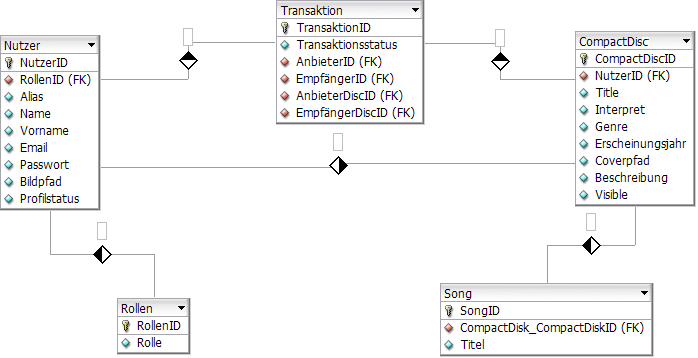
\includegraphics[height=7cm]{images/ERTauschbooerse.png}
	\caption[Erste Version des ER-Modells f�r die CD-Tauschb�rse]{Erste Version des ER-Modells f�r die CD-Tauschb�rse}
	\label{fig:ER}
\end{figure}

Um eine Arbeitsgrundlage zu erstellen, wurde zuerst das Datenbankschema in Rails erstellt. Rails bietet dazu einen ActiveRecord an der als Layer zwischen dem SourceCode und der Datenbank fungiert. Dazu wird f�r jede Tabelle ein Modell erstellt. Zwar bietet Rails die M�glichkeit mit einem einzigen Kommando sowohl Modell, Controller und Views zu generieren. Davon wurde aber kein Gebrauch gemacht, da es entschieden wurde die Anwendung Schritt f�r Schritt zu entwickeln, um gr��tm�gliche Kontrolle zu erreichen. Es wurden f�nf Modells mit dem Kommando \textit{rails generate model <Bezeichnung>} erstellt. Das einzige was Rails noch macht ist f�r jedes Modell eine TestKlasse anzulegen. Nachdem alle erforderlichen Modelle angelegt wurden, konnte das Schema in die Datenbank migriert werden mit dem Ziel das modellierte Schema zu testen. Rails bietet dazu eine geeignete Testumgebung an. Hierzu wurden die Unit Tests entwickelt. Auf diese Art und Weise wird es sichergestellt, dass das Datenbankschema einwandfrei funktioniert ohne auch daf�r eine einzige Zeile Code geschrieben (z.B. f�r Controller oder View) zu haben. Basierend auf einer funktionierenden Datenbank werden die einzelnen Views und Controller integriert. Die �nderungen im Datenbankschema k�nnen nachtr�glich ohne Probleme integriert werden.

Nach der Bekanntgabe der �nderungen im Pflichtenheft, wurde sofort ersichtlich, dass das erstellte Datenbankschema modifiziert werden soll. F�r die Realisierung eines Austauschs mit mehreren CD's, wurde die n:m Beziehung bei den Transaktionen hinzugef�gt. Dabei wurden zwei zus�tzliche Tabellen mit aufgenommen. Dar�ber hinaus sind weitere Attribute f�r die Realisierung andrer Funktionalit�ten hinzugekommen. Folgende Abbildung stellt das endg�ltige Schema der Datenbasis dar:

\begin{figure}[ht]
\centering
		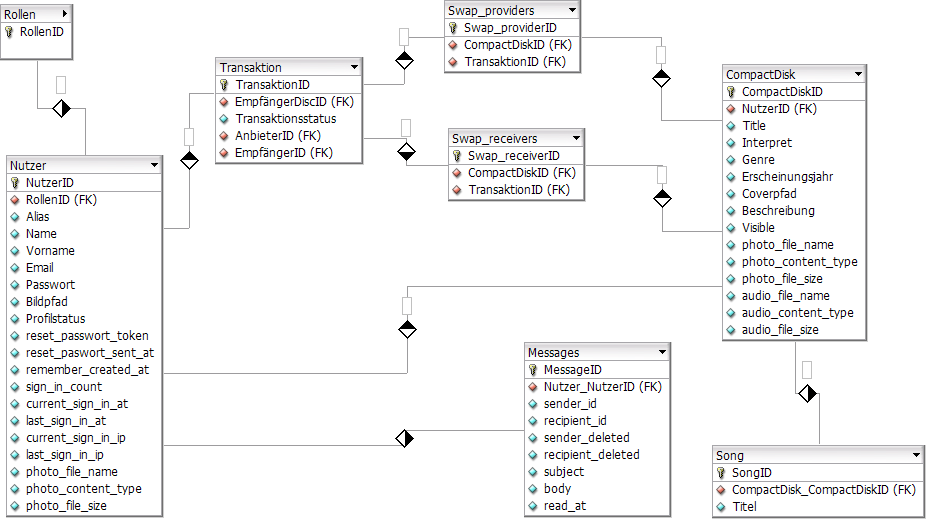
\includegraphics[height=8cm]{images/ermnew.png}
	\caption[ER-Modell f�r die CD-Tauschb�rse]{ER-Modell f�r die CD-Tauschb�rse}
	\label{fig:ER2}
\end{figure}

\section{Realisierung der Funktionalit�t}
\label{sec:Realisierung der Funktionalit�t}

Die Grundlage der Anwendung, wurde mit dem Erstellen von Modells, geschaffen. F�r die Realisierung der geforderten Funktionalit�t wurden Gedanken �ber die ben�tigten Controller und Views gemacht werden. Controller werden in Rails mittels des Kommandos \textit{rails generate controller <Bezeichnung>} erstellt. Zu jedem Controller k�nnen mehrere Views geh�ren. In der Datei \textit{routes.rb} wird definiert welche Methode im Controller auszuf�hren ist, wenn eine bestimmte View im Browser aufgerufen wird. Des Weiteren wurden, f�r jede Anforderung im Pflichtenheft, User Stories geschrieben, um die Aufgaben besser zu verteilen. 

\subsection{Benutzerverwaltung}
\label{sec:Benutzerverwaltung}

Als erstes wurde untersucht, ob eine eigene Implementierung aufwendig ist, oder nicht. Hierzu wurde mittels eines Tutoriell die Benutzerverwaltung realisiert. Es muss gesagt werden, dass diese Implementierung nur ein Grundger�st der Autorisierung-Funktionalit�t darstellt und mehrere Sicherheitsrisiken ausweist. Aus diesem Grund wurde entschieden ein sicherer und gut dokumentierter Plug-In zu verwenden.

F�r diese Zwecke wurden mehrere Plug-Ins evaluiert, sodass wir auf die Entscheidung gekommen sind Devise zu verwenden. Diese Erweiterung bietet eine flexible L�sung zur Benutzerauthentifizierung f�r Rails und besteht aus 12 Modulen wie zum Beispiel:

\begin{enumerate}
	\item Confirmable
	\item Authenticatable
	\item Recoverable	
	\item Registerable	
	\item Rememberable (Cookies)
	\item Validatable
	\item Encryptable
	\item ...
\end{enumerate}

Alle diese Module sind nach dem MVC-Prinzip implementiert und k�nnen nach Bedarf kombiniert werden. Dadurch wird erreicht, dass jede Applikation nur die geforderten Funktionalit�ten hat. Die Installation dieses Plug-Ins ist entsprechend einfach und kann nur in wenigen Schritten realisiert werden:

\begin{enumerate}
	\item Gemfile: gem 'devise' 
	\item \textit{bundle install} -->  fehlende Gems installieren 
	\item \textit{rails generate devise:install} --> Plug-In installieren 
  \item Migration(en) anpassen oder mit \textit{rails generate device user} ein neues Modell erstellen
  \item Migrationen ausf�hren \textit{rake db:migrate}
\end{enumerate}

Da das Plug-In \textit{Devise} nur die Benutzerauthentifizierung gew�hrleistet wurde nach einem Rollenverwaltungstool recherchiert, um ein Rollenmanagement zu realisieren, dadurch den Nutzern unterschiedliche Rechte zu geben und dadurch die Anwendung zu sch�tzen. Hierzu wurde \textit{CanCan} analysiert und getestet.  \textit{CanCan} ist ein Plug-In, welches auf Device aufgebaut wird. Nach der Installation wird eine neue Klasse activity angelegt, die nach Bed�rfnissen konfiguriert werden soll. Somit bietet diese Erweiterung die Definition von mehreren Gruppen (Gast, Benutzer, Admin) sowie eine einfache und vor allem schnelle Rechtevergabe.

\subsection{Compact Discs}
\label{sec:Compact Discs}

F�r die Darstellung von mehreren CD's auf einer Seite wurde das Plug-In \textit{WillPaginate} f�r Rails untersucht und implementiert. Denn wenn die CD's einem Benutzer angezeigt werden, ist es nicht erw�nscht immer alle CD's auf einer Seite zeigen, da die Anzahl sogar mehrere hundert CD's betragen kann. Einerseits w�re diese Darstellung zu un�bersichtlich und zum Anderen ist auch die Zeit die der Server f�r die Antwort der Anfrage ben�tigen w�rde w�re viel zu lang. Daher ist es sinnvoll, die CD's auf mehrere Seiten aufzuteilen. Genau das macht \textit{WillPaginate}. Es muss lediglich definiert werden wie viele CD's in der View gezeigt werden m�ssen. Sind mehr CD's vorhanden als auf der Seite dargestellt, sind diese �ber weitere Seiten (1,2,...) erreichbar.

\subsection{Tausch-Transaktionen}
\label{sec:Tausch-Transaktionen}

F�r die Realisierung der Hauptfunktionalit�t wurde �berlegt wie der Austausch von CD's erfolgen kann. Da diese Funktion mit einem Plug-In bzw. durch die Verwendung eines internen Messaging-Systems realisiert werden sollte, wurde ermittelt welche davon in Frage kommen. Es wurde entschieden ein Plug-In f�r die interne Kommunikation bzw. den Nachrichtenaustauch auszuw�hlen und f�r unsere Zwecke zu verwenden. Hierzu wurden mehrere Plug-Ins recherchiert und mit einander verglichen:

\begin{itemize}
	\item has-messages
	\item simple-messaging
	\item simple-private-message
\end{itemize}

Diese Plug-Ins wurden hinsichtlich der Funktionalit�t, Dokumentation, Verbreitung sowie der Weiterentwicklung bzw. Support untersucht. Es wurde herausgestellt, dass simple-private-message die erforderlichen Funktionalit�ten zur Verf�gung stellt und zu den wenigsten Plug-Ins geh�rt, die fertiggestellt sind und auch mit der Rails Version 3.0.1 kompatibel sind. Dar�ber hinaus wurde die Funktionalit�t anhand eines Tutoriells �berpr�ft. Die Installation dieses Plug-Ins ist sehr einfach und ben�tigt lediglich drei Schritte:

\begin{enumerate}
	\item Gem File anpassen + \textit{bundle install}
	\item \textit{rails generate simple-private-messages:model User Message}
	\item Controller ''Transaktionen'' erstellen
\end{enumerate}

Um die Implementierung der Funktionalit�t zu vereinfachen wurde die Kommunikation visuell dargestellt. Somit konnten alle Anforderungen hinsichtlich der Sicherheit erf�llt werden.

\begin{figure}[ht]
\centering
		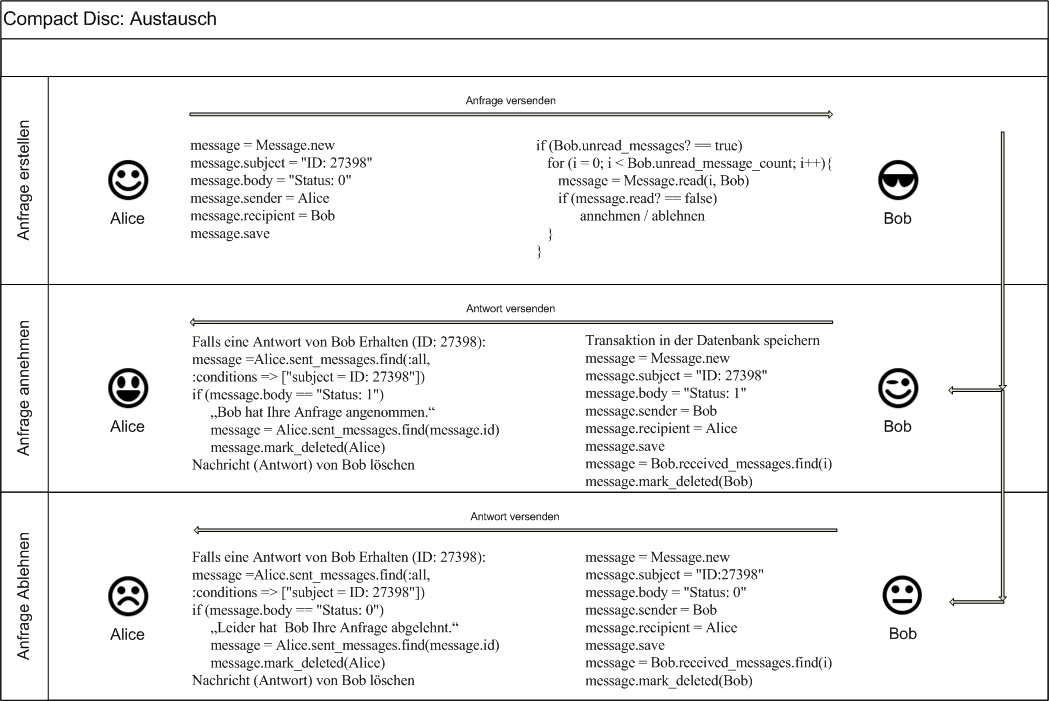
\includegraphics[height=9cm]{images/Transaktionen.png}
	\caption[Verlauf CD-Tauschb�rse]{Verlauf CD-Tauschb�rse}
	\label{fig:ER}
\end{figure}

Bei der Implementierung dieser Funktionalit�t wurde sowohl auf die Korrektheit, als auch auf die Sicherheit des Transaktionsaustauschs geachtet. Falls die Anfrage abgelehnt wird, werden die zugeh�rigen Nachrichten gel�scht, ohne einen Datenbank Eintrag zu machen. Wenn der Austausch akzeptiert wird bzw. zustande kommt, werden die CDs ausgetauscht und die gesamte Transaktion in der Datenbank gespeichert. Somit besteht die M�glichkeit es zu jeder Zeit zu pr�fen, wer mit wem welche CD's getauscht hat. Am 1. Dezember erfolgten die �nderungen des Pflichtenhefts, so dass es erforderlich war die Vorgehensweise etwas zu Ver�ndern. Dar�ber hinaus wurden weitere Tabellen in die Datenbank aufgenommen.

Wie im Pflichtenheft gew�nscht ist, wurde der Austausch von CDs durch ein internes Messaging-System realisiert. Bei der Implementierung wurde darauf geachtet, dass die Transaktionen sicher durchgef�hrt werden, sodass in der vordefinierten Reihenfolge die Datenbankeintr�ge gemacht werden und keine Information verloren gehen k�nnen. Nun wurde der Fall nicht ber�cksichtigt, falls ein Benutzer die CD l�scht, die immer noch im Anfragemodus befindet. Nach einer Diskussion wurden zwei M�glichkeiten �berlegt:

\begin{enumerate}
	\item Wenn eine CD gel�scht wird, wird es gepr�ft ob es die Anfragen mit dieser CD gibt, oder nicht. Wenn das nicht der Fall ist, kann die CD gel�scht werden. Wenn allerdings eine Anfrage besteht, wird diese automatisch abgebrochen und die Beteiligten erhalten eine Nachricht.
	\item Die einfachere Methode ist es das L�schen zu verbieten solange eine Anfrage besteht. D.h. bevor eine CD gel�scht werden kann, m�ssen alle zugeh�rigen Abfragen gel�scht werden.
\end{enumerate}

\subsection{Sonstige Anforderungen}
\label{sec:Sonstige Anforderungen}

Dar�ber hinaus wurde die Anforderung erf�llt, den Austausch mit Drag and Drop zu entwickeln. Die Drag and Drop Funktionalit�t wurde durch jQuery realisiert. Daf�r wurde die View, auf der der CD-Tausch vollzogen wird, in vier Bereiche (DIV-Elemente) unterteilt. Alle vier Bereiche bzw. alle darin enthaltenen Elemente (CDs) bieten die Drag und Drop Funktion. Daf�r werden die von jQuery bereitgestellten Methoden draggable und droppable genutzt. Diese Methoden werden den einzelnen Div-Elementen zugewiesen. Zur Identifizierung und Nutzung der Div-Elemente innerhalb der jQuery Javascript Datei, dient die eindeutige ID, welche jedes Element besitzt.

\begin{figure}[ht]
\centering
		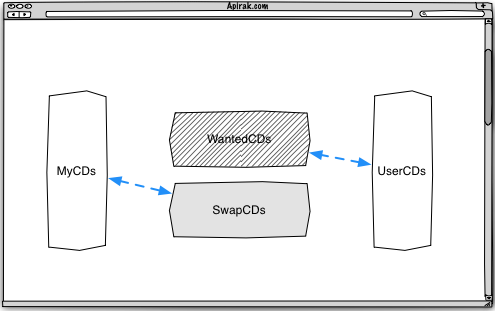
\includegraphics[height=7cm]{images/draganddrop.png}
	\caption[Drag nad Drop Funktionalit�t]{Drag nad Drop Funktionalit�t}
	\label{fig:ER}
\end{figure}


Die Grafik zeigt den Schematischen Aufbau der Seite. Die �u�eren Bereiche zeigen alle CDs, des aktuell angemeldeten Benutzers (MyCDs) und des Tauschpartners (UserCDs), an. Diese CDs k�nnen dann in einen der mittleren Bereiche gezogen werden (WantedCDs oder SwapCDs).
Um sicherzustellen, dass die Bereiche WantedCDs und SwapCDs nur nur Elemente aufnehmen welche aus einem bestimmten Div-Container kommen, wurden Beschr�nkungen in jQuery definiert. Dies geschieht durch die Option accept, welches die droppable Elemente bieten. 

\$('\#swapCDs').droppable({

	accept: ''\#myCDs > img''
	
});

Wie im Beispiel zu sehen, akzeptiert das Element swapCDs nur img-Elemente aus dem MyCDs Bereich. Dadurch kann verhindert werden, dass ein Nutzer CDs aus der Sammlung des Tauschpartners in beide Bereiche (WantedCDs und SwapCDs) zieht und somit eine Anfrage erstellen kann, ohne eine CD aus seiner eigenen Sammlung zum Tausch angeboten zu haben.
Die IDs der CDs, die auf dem Swap oder Wanted Bereich gezogen werden, werden in einem Array gespeichert (F�r jeden Bereich ein separates Array). Falls ein Element wieder  aus einem der mittleren Bereiche entfernt wird, wird es auch aus dem entsprechenden Array gel�scht. Sobald eine Anfrage Abgeschickt werden soll, werden die Werte des Arrays ausgelesen und als Parameter an den Link zur Action im Controller angef�gt. 

\section{Graphical User Interface}
\label{sec:Graphical User Interface}

In der ersten Woche wurden erste Entw�rfe zum Design der CD-Tausch-Plattform erstellt. Diese wurden w�hrend der Teammeetings in Form von einfachen Skizzen in analoger Form festgehalten und im Anschluss mittels Adobe Photoshop als Mockups ausgearbeitet. Basierend auf diesen Entw�rfen wurde ein HTML5 Layout mittels CSS-Stylesheet erstellt.

\begin{figure}[ht]
\centering
		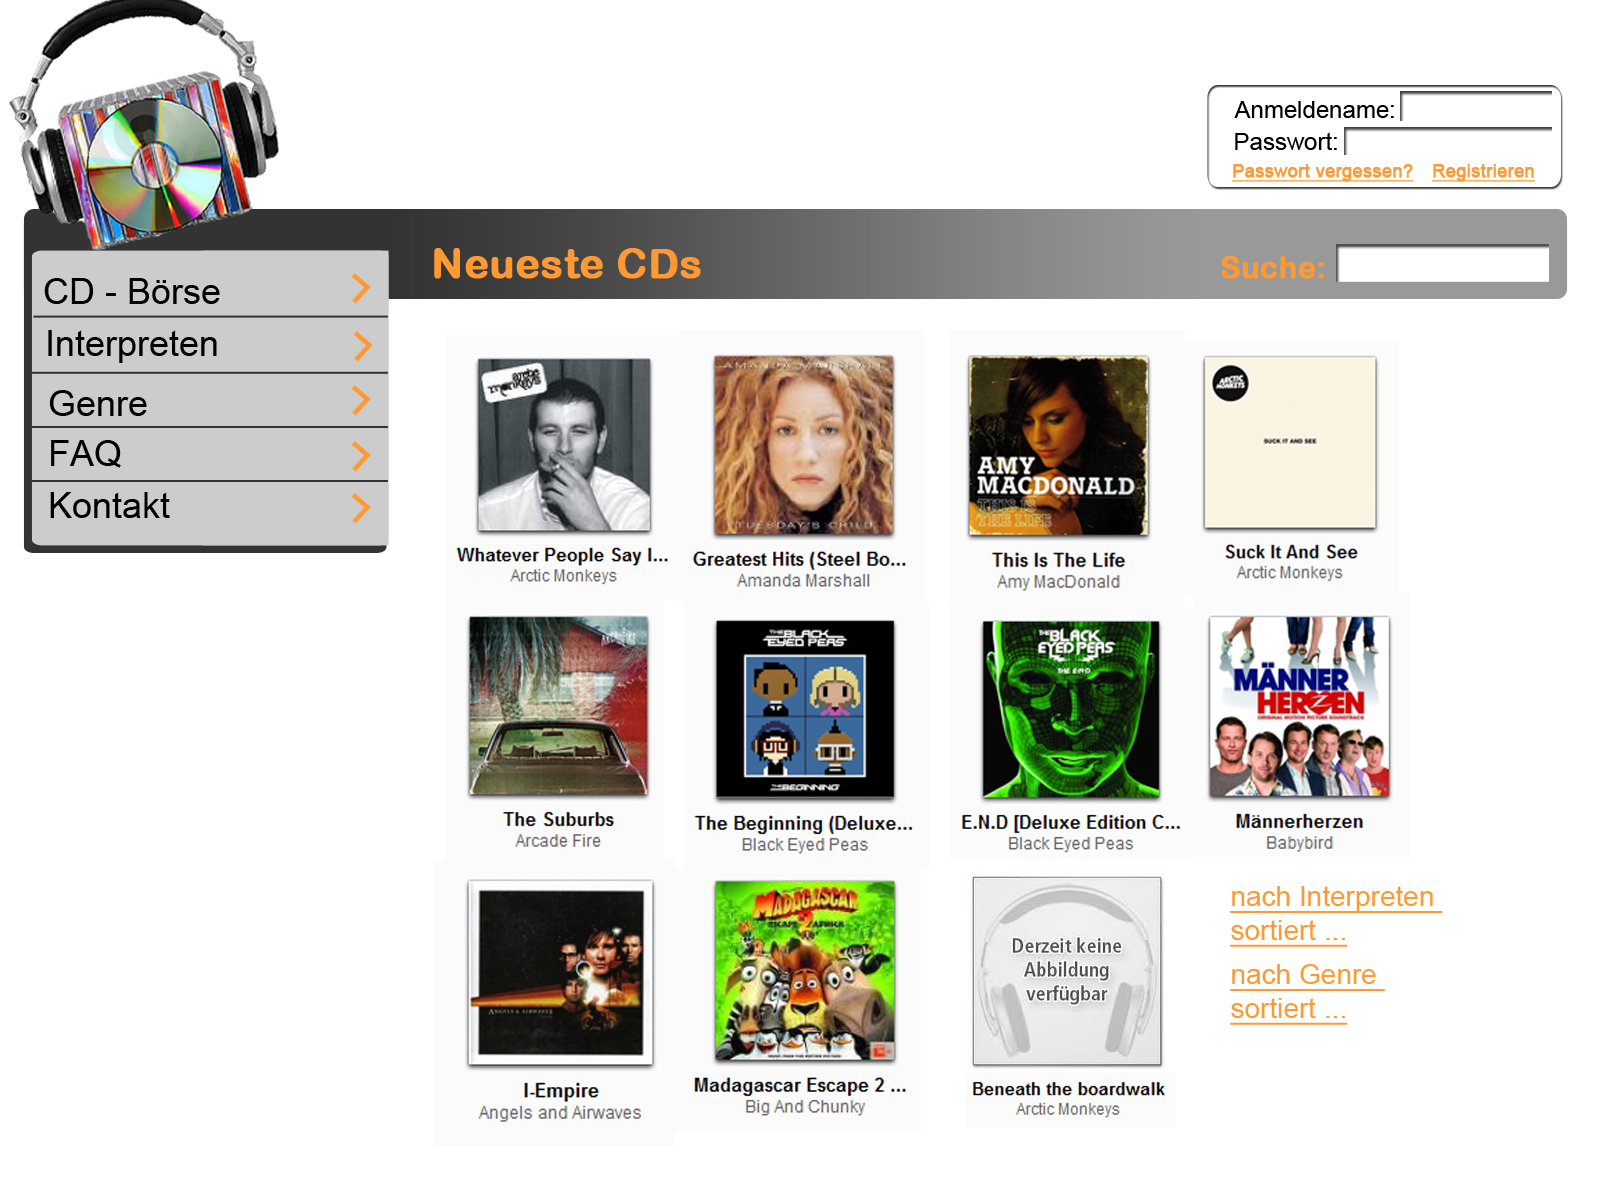
\includegraphics[height=7cm]{images/design1.jpg}
	\caption[Design 1]{Design 1}
	\label{fig:ER}
\end{figure}

Im Laufe der Entwicklung wurde das Design noch einmal �berarbeitet, da es dem ersten Entwurf an Struktur fehlte. Im Team wurde entschieden dieses noch einmal zu �berarbeiten und daf�r ein Template zu nutzen, um eine einheitliche Darstellung zu erzielen. Zur engeren Auswahl standen Blueprint CSS, 960gs und Bootstrap. Die Entscheidung fiel auf Bootstrap von Twitter. Bootstrap ist ein spezielles Toolkit, das im Wesentlichen ein HTML- und CSS-Template bereitstellt, in das Twitter seine Erfahrungen einflie�en lie�. Webentwickler, die Bootstrap in ihr Frontend einbinden, sollen so auf praxiserprobte Frontend-Entwurfsmuster zur�ckgreifen k�nnen und
unter anderem ohne gr��eren Aufwand ein Grid-System einbinden, das bei Twitter erprobte Styling f�r typographische Elemente �bernehmen, Formulare und Buttons verwenden oder ihre Seiten mit Modal-Boxen, Tooltipps und Popovers erg�nzen. Dieses Template enth�lt viele L�sungsans�tze zur Realisierung von Javascript Effekten. So auch die von Tooltips und Popover. F�r die Realisierung von den Tooltips haben wir die Funktion .popover von Bootstrap verwendet. Dort wird in einer Variable, der anzuzeigenden Text an. Dieser wird in einem Popover angezeigt, wenn mit dem Mauszeiger �ber die verlinkte Region gefahren wird.

\begin{figure}[ht]
\centering
		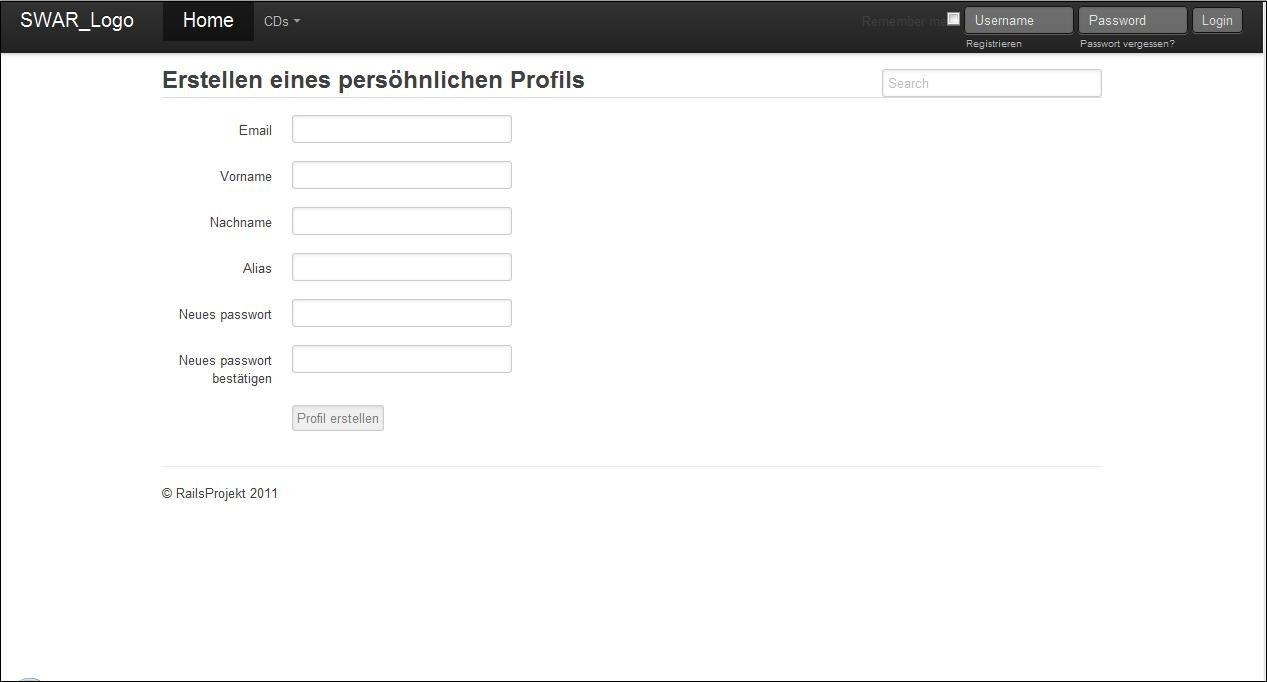
\includegraphics[height=7cm]{images/design2.jpg}
	\caption[Design 2]{Design 2}
	\label{fig:ER}
\end{figure}

\section{Internationalisierung}
\label{sec:Internationalisierung}

Da es vor der Bekanntgabe der �nderungen nicht bekannt war, welche Funktionalit�ten hinzukommen, wurden Gedanken �ber eine Internationalisierung der Anwendung gemacht. Unser Team ist davon �berzeugt, dass jede gute Webanwendung mehrere Sprachen unterst�tzen soll, um eine m�glichst gro�e Nutzerzahl zu erreichen.

Das Einbinden von verschiedenen Sprachen erfolgt in Rails �ber eine \textit{localize} Datei. Diese hat den Namen der Sprache, also z.B.: de.yml. In den Views werden nun Variablen f�r die Bezeichnungen eingetragen. In der \textit{localize} Datei steht dann zu jeder Variablen die entsprechende �bersetzung. F�rs erste haben wir uns auf die deutsche Sprache beschr�nkt, da es hierzu keine Anforderungen gab. Am Ende der Entwicklung ist es sehr einfach andere Sprachen zu implementieren. Die localize Datei muss dazu nur kopiert werden. Die Neue Datei bekommt den Namen der neuen Sprache z.B.: en.yml. Nun m�ssen alle Bezeichnungen �bersetzt werden, sodass dadurch die Lokalisierung bzw. Internationalisierung realisiert werden kann. 

Damit Rails auch wei�, f�r welche Komponenten eine Lokalisierung zur Verf�gung steht, muss diese noch in den jeweiligen Controllern ein gepflegt werden. Dazu m�ssen auch f�r alle Routen entsprechende Eintr�ge vorgenommen werden. Dabei z�hlt auch welche Sprachen unterst�tzt werden sollen. Das sind aber nur einmalige Anpassungen, die wenig Zeitaufwand ausweisen. Herauszufinden welche Sprache der Benutzer hat kann �ber die HTTP Header geschehen. Alternativ kann der Benutzer selber eine Sprache ausw�hlen. Eine Sprache kann auch als Standard gesetzt werden wenn keine Informationen vorliegen. Dabei wurde herausgestellt, dass eine Anwendung zu internationalisieren erfordert nur einmalig ein wenig Aufwand. Danach kann man aber leicht die Anwendung um jede gew�nschte Sprache erweitern.

%\chapter{Untersuchung der Technologien}
\label{sec:Untersuchung der Technologien}

... 

\section{Auswahl von Funktechnologien}
\label{sec:Auswahl von Funktechnologien}

...

\section{Festlegung der Untersuchungskriterien}
\label{sec:Festlegung der Untersuchungskriterien}

...

\section{Messwerterfassung}
\label{sec:Messwerterfassung}

...

\section{Auswertung der Messergebnisse}
\label{sec:Auswertung der Messergebnisse}

...

\section{Vergleich der Technologien}
\label{sec:Vergleich der Technologien}

...
%\chapter{Konzeption und Implementierung eines Prototyps}
\label{sec:Konzeption und Implementierung eines Prototyps}

...

\section{Entwicklungsumgebung und Systemvoraussetzung}
\label{sec:Entwicklungsumgebung und Systemvoraussetzung}

...

\section{Konzept}
\label{sec:Konzept}

...

\section{Implementierung eines Prototypen}
\label{sec:Implementierung eines Prototypen}

...
\chapter{Zusamenfassung}
\label{sec:Zusammenfassung}
In diesem Kapitel fassen die Projektteilnehmer ihre Erfahrungen nach dem Projekt zusammen.
\section{Antonia Ziegler}
Insgesamt würde ich Ruby on Rails als ein sehr modernes und zukunftsorientiertes Framework mit einer grossen Community bezeichnen.
Die Entwicklungsumgebung lässt sich insgesamt gut auf verschiedenen Betriebssystemen aufsetzen. 
Wenn man sich an das gegebene MVC Prinzip hält, ist ein Ruby on Rails Projekt gut erweiterbar und wartbar. 
Was mir am besten gefällt ist die Möglichkeit, oft ziemlich einfach, Plugins einzubinden. Auf Grund der grossen Community gibt es viele Open Source Plugins, welche Funktionen bieten, wie z.B. die Pagenavigation. Diese wiederum sind gut erweiterbar oder anpassbar.
\section{Christian Sandvoss}
Ich finde, das man Railsls sehr gut verwenden kann um auch umfangreiche Webanwendung zu realisieren. Rails stellt ein Grundsystem bereit, das durch viele Pugins erweiterbar ist. Allerdings muss man dabei darauf achten ob das Plugin zur genutzten Rails Version kompatibel ist oder überhaupt noch weiter entwickelt wird. Des weiteren ist bei einigen Plugins die Dokumentation sehr kurz gehalten. Die Dokumentation von Rails ist dagegen, wie ich finde, sehr gut. Es gibt Tutorials zum Einstieg sowie eine aktive Community. Neu für mich war die Arbeit mit JavaScript bzw. JQuery. Es war für mich sehr interessant das Zusammenspiel von verschiedenen Sprachen (Ruby, HTML/CSS, JavaScript) kennenzulernen.

\section{Alexander Miller}
Durch die Realisierung des Projektes konnte ich persönlich feststellen welche Vor- und Nachteile Rails ausweist. Die Verwendung von Rails, können sogar komplexe RIA Web-Anwendungen realisiert werden. Die wesentlichen Prinzipien dieses Frameworks sind Konvention over Configuration und MVC Prinzip. Im Allgemeinen ist Rails sehr gut dokumentiert und hat eine grosse und vor allem aktive Community. Der Umfang an Möglichkeiten ist enorm gross, so dass viele Funktionalitäten problemlos implementiert werden können. Darüber hinaus besteht die Möglichkeit viele Module als Plug-Ins zu integrieren. Der Prozess der Integration von PlugIns ist trivial wenn dieser ausreichend Dokumentiert ist. Leider sind manche PlugIns schlecht dokumentiert, so dass die Auseinandersetzung manchmal viel Zeitaufwand erfordert. Insgesamt bin ich mit dem Framework sehr zufrieden, so dass es nichts dagegen spricht für die Realisierung einer weiteren Web-Applikation Rails zu verwenden.
\section{Christian Bunk}
Ich muss sagen das sich meine Einstellung zu Webframeworks sehr geändert hat. Ich hatte früher nie Lust auf Webentwicklung, da mir Frameworks wie Spring und Struts viel zu kompliziert, zu sperrig, ja sich einfach nicht schön an die Entwicklung von Web Applicationen angefühlt haben. Aber mit Ruby on Rails hat sich das sehr geändert. Schon die Programmiersprache Ruby macht das schreiben von Programmen sehr angenehm. Es ist eine elegante und moderne Sprache. Darauf ein Webframework aufzubauen erscheint nur logisch. Mit Ruby on Rails hat man das Gefühl das alles gut durchdacht ist. Durch das Prinzip Convention over Configuration ist es möglich mit wenig aufwand viel zu erreichen. Alles ist da wo es sein soll und wo es hingehört. Hält man sich an bestimmte Regeln des Frameworks macht die Entwicklugn einfach Spass. Das bedeutet aber nicht das die Entwicklung leicht ist. Im Gegenteil Rails ist ein Framework mit sehr grossem Funktionsumfang. Selbst in den 3 Monaten unserer Entwicklung haben wir in vielen Bereich nur an der Oberfläche gekratzt. Rails bietet eine wunderbare und umfangreiche Dokumentation. Aber um hier hinter alle Konzepte zu steigen braucht es einfach Zeit. Rails bietet mit Erweiterungen durch Module oder Plugins die Möglichkeit Funktionen in seine Webanwendung zu integrieren. Das ist gut solange man nicht mehr Funktionalität braucht als die jeweiligen Plugins bieten. Schwierig wird es wenn man doch eigene oder zusätzliche Funktionen benötigt. Dann muss man versuchen um das Plugin herum zu entwickeln, da meist genaue Dokumentation für die sehr speziellen Fälle fehlen. Mit Rails habe ich auch das Routing, also das mappen von URLs auf bestimmte Methoden in einem Controller, besser verstanden. Das Konzept von Active Record hat mich sehr überzeugt, da hier SChnittstellen und Datenbanken optimal verschmelzen und nicht mehr an jeder Stelle im Code die Datenbank kryptisch ausgelesen oder konfiguriert werden muss. Es wird einfach ein Model definiert, über welches man die Attribute definiert. Diese werden dann automatisch in die Datenbank eingetragen. Rails eignet sich sehr gut für verteilte Entwicklung. Es werden weder Lizenzen benötigt, noch wird dem Programmierer eine IDE aufgezwungen. Alles kann in einem einfachen Texteditor entwickelt werden. Mehr als einen Browser und ein Terminal braucht man dann nicht. Entgegen manchen Vorstellungen das Rails einfach sei muss ich wiedersprechen. MAn braucht viel Zeit um die Konzepte sich zu eigen zu machen. Auch braucht man (wie bei jedem anderen Framework) Zeit um Funktionalitäten zu programmieren. Ich denke eh nicht das man Frameworks nach leichter und schwerer Kategorisieren kann. Ich denke das ich mit Rails wertvolle Erfahrungen gesammelt habe die mir im meinem späteren Berufsleben nützlich sein werden. Ich denke auch das ich mit Rails noch öfter in Zukunft in berührung kommen werde. Rails muss man einfach erlebt haben.
% Literaturverzeichnis:
%\bibliography{C:/literatur}

%Anh�nge:
\appendix

\chapter{Anhang}
\label{sec:Anhang}

\section{Aufgabenstellung}
\label{lst:Aufgabenstellung}


\includepdf[scale=0.88, pages=-, pagecommand={\thispagestyle{headings}}]{pdfs/aufgabe.pdf}

%% Selbst�ndigkeitserkl�rung:
\chapter*{Selbst�ndigkeitserkl�rung}
\label{sec:Selbstaendigkeitserklaerung}
%\addcontentsline{toc}{chapter}{Selbst\"andigkeitserkl\"arung}
\subsection*{Erkl�rung}
\vspace{3ex}
Ich erkl�re, dass ich die vorliegende Seminararbeit selbst�ndig und nur unter Verwendung der angegebenen Quellen und Hilfsmittel angefertigt habe.

\vspace{6ex}
\begin{tabular}{llr}
 \hspace{4cm} & \hspace{1cm} Berlin, den &  \hspace{4cm} \\ \cline{1-1} \cline{3-3}
\end{tabular}


%--------------------------------------
%   Dokumentenende
%--------------------------------------
\end{document}